\chapter{Central Dogma}

\section{Base Pairing and the Double Helix}
The chemical structure of each base allows it to match up with another.
\begin{itemize}
    \item Guanine - Cytosine (G - C): Three Hydrophone bond
    \item Adenine - Thymine (A - T): Two Hydrophone bond
    \item Start of the sequence: 5' end
    \item End of the sequence: 3' end
\end{itemize}

\section{Ribonucleic acid (RNA) and Deoxribonucleic acid (DNA)}

DNA and RNA are composed of similar monomer building blocks. They provides ultra high density base-4 memory.

\begin{figure}[h]
\centering
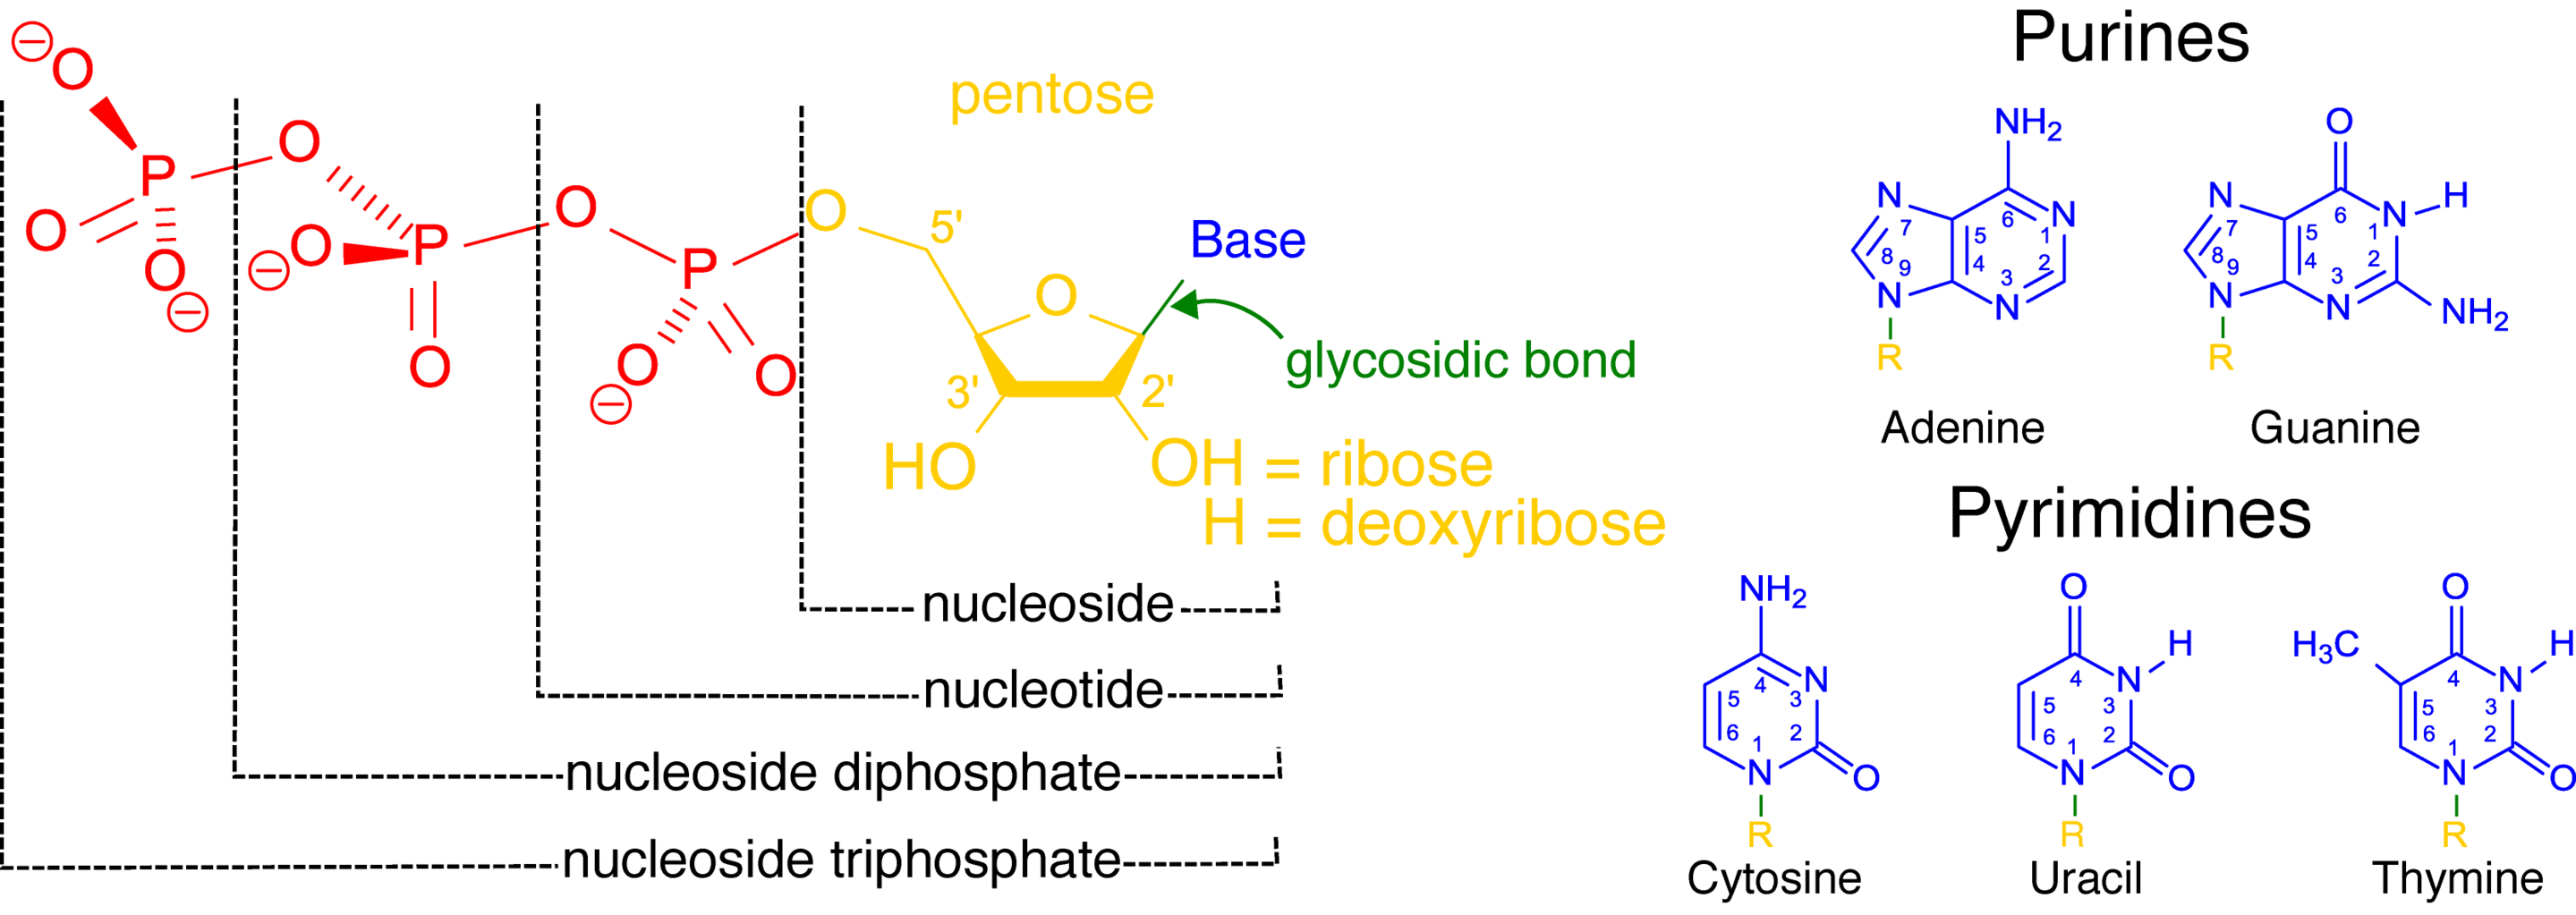
\includegraphics[width=1\textwidth]{images/Nucleotides.png}\\[.2in]
\caption{RNA and DNA} 
\end{figure}

\begin{itemize}[noitemsep]
    \item \bd{A} Adenine
    \item \bd{G} Guanine
    \item \bd{C} Cytosine
    \item \bd{U} Uracil
    \item \bd{T} Thymine
\end{itemize}
Nucleoside = Sugar + Base (the information carrier)
\begin{itemize}
    \item DNA: sugar is deoxyribose\footnote{a sugar derived from ribose by replacement of a hydroxyl group by hydrogen.}; bases are A,C,G,T - relatively stable.
    \item RNA: sugar is ribose\footnote{a sugar of the pentose class which occurs widely in nature as a constituent of nucleosides and several vitamins and enzymes.}; bases are A,C,G,U - relatively unstable.
\end{itemize}
The nucleotide triphosphate forms are the building block.

\section{RNA structural diversity}
\udl{A single-stranded RNA molecule can base-pair with itself}
to form structures that are biochemically important. It is quite possible that RNA molecules or something similar are the origin of life.\\[.2in]
Examples: Hammerhead ribozyme\footnote{an RNA-cutting RNA enzyme} and transfer RNA.

\section{Amino acid structure}
\begin{figure}[h]
    \centering
    \chemfig{N(-[3]H)(-[5]H)-C(-[2]R)(-[6]H)-C(=[1]O)(-[-1]OH)}
    \caption{Amino acid structure}
\end{figure}
\begin{itemize}[noitemsep]
    \item R-group (side chain)  
    \item Amino group: N terminus
    \item Alpha carbon
    \item Carboxyl group: C terminus
\end{itemize}
Amino acids: modular protein sub-units: 20 amino acid structures.
\begin{enumerate}[itemsep=0mm]
    \item Amino acids with hydrophobic side chains
    \item Amino acids with hydophilic side chains
    \item Amino acids with intermediate side chains
\end{enumerate}

\section{The peptide bond}
The N terminus (Amino terminus) is the start of a protein and the C terminus (Carboxy terminus) the end.
\begin{scheme}[h]
    \centering
    \schemestart
        $2$ \chemname{
            \chemfig{N(-[3]H)(-[5]H)-C(-[2]R)(-[6]H)-C(=[1]O)(-[-1]OH)}
        }{Amino acid}
        \arrow(.mid east--.mid west){<=>[Dehydration]}
        \chemname{
            \chemfig{N(-[3]H)(-[5]H)-C(-[2]H)(-[6]R)-C(=[2]O)-N(-[-2]H)-C(-[2]H)(-[6]R)-C(=[1]O)(-[-1]OH)}
        }{Pipetide group}
        \+
        \[ \text{H}_2\text{O} \]
    \schemestop
    \caption{The condensation reaction to generate a pipetide group}
    \label{scm:tsester}
\end{scheme}


\section{Protein structural hierarchy}

\bd{Primary structure}: sequence of amino-acids: determines the final form and function (peptide bonds)\\[.1in]
\bd{Primary structure}: sequence of alpha-helices, beta-sheets (hydrogen bonding)\\[.1in]
\bd{Tertiary structure}: overall 3D fold (disulphide bonds, ionic bonds, hydrogen bonds...)\\[.1in]
\bd{Quaternary structure}: complex of proteins

\section{Information flow: the Central Dogma of molecular biology}
Francis Crick (1958) raised the idea that the information flows from the DNA to RNA, and then to the Proteins.
\begin{figure}[h]
\centering
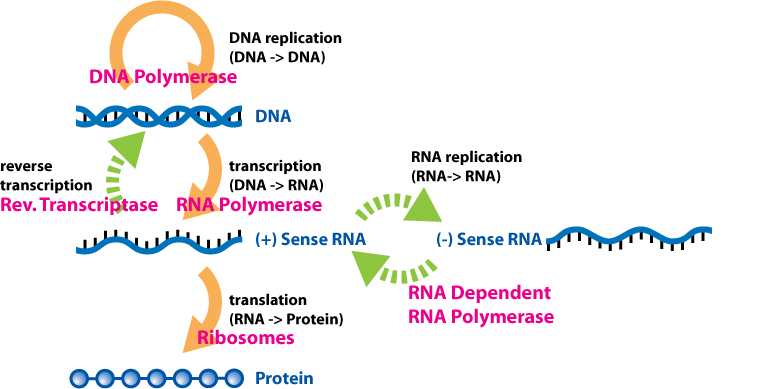
\includegraphics[width=0.8\textwidth]{images/Extended_Central_Dogma_with_Enzymes.jpg}\\[.2in]
\caption{Demonstration of Central Dogma} 
\end{figure}
\begin{enumerate}
    \item DNA replication via DNA Polymerase\footnote{catalyse the synthesis of DNA molecules from nucleoside triphosphates, the molecular precursors of DNA} (DNA $\rightarrow$ DNA)
    \item Transcription via RNA polymeras\footnote{an enzyme that synthesises RNA from a DNA template} (DNA $\rightarrow$ RNA)
    \item Translation via Ribosomes\footnote{Ribosomes link amino acids together in the order specified by the codons of messenger RNA (mRNA) molecules to form polypeptide chains.} (DNA $\rightarrow$ Protein)
\end{enumerate}

\subsection{DNA polymerase}
\begin{itemize}
    \item DNA replication is catalysed by DNA polymerase.
    \item Polymerisation is in the 5' $\rightarrow$ 3' direction.
    \item DNA polymerase starts from an existing 3'-hydroxyl group, i.e. it needs a "\textit{primer}".
    \item The primer can be a \udl{synthetic DNA molecule} that anneals to a template through \textit{complementary base pairing}.
\end{itemize}
\newpage
\subsection{Transcriptions and Translations}
\bd{Transcription} \\ [.1in]
Transcription is re-writing in a similar alphabet.
\begin{itemize}
    \item Catalysed by RNA polymerase enzyme from 5' to 3' direction.
    \item Template strand is the bottom strand (\textit{coding strand}).
    \item RNA uses Uracil (U) instead of T.
    \item RNA has a 2'hydroxyl group (so ribose not deoxyribose)
    \item The RNA molecule is called a transcript. The transcript of a protein-coding RNA is called a messenger RNA (mRNA).
\end{itemize}
Convention: for a gene drawn, we write the sequence of the \udl{top strand}. We need to reverse-complement genes on the bottom strand.\\[.2in]
\bd{Translation} \\ [.1in]
Translation is recoding: one \textit{codon} = 3 bases. Therefore, 64 codons map to 20 amino acids + 3 stop codons. \udl{Translation is carried out by the ribosome.} The ribosome is a giant RNA/protein complex that has two subunits.
\begin{itemize}
    \item The mRNA is read 5' $\rightarrow$ 3'.
    \item The protein is sythesised N terminus $\rightarrow$ C terminus.
    \item The redundancy of 3 bases is removed by a multiple-to-one mapping from codons to amino acids.
    \item The tRNA carries the Amino acid and with \udl{anticodon loop} on the other side which matches the mRNA. 
\end{itemize}
Enzymes called \udl{amino-acly rRNA synthetases} 'charge' tRNAs by attaching the correct amino-acid for the anticodon.
\begin{itemize}
    \item Certain tRNAs recognise more than one codon by means of the last base "wobbling" (forming atypical base pairs).
    \item tRNA synthetases have been evolved that can mis-charge tRNAs with exotic amino-acids.
\end{itemize}
Epigenetics and prions make the picture more complicated but the central dogma is still central to life.
